% #######################################
% ########### FILL THESE IN #############
% #######################################
\def\mytitle{EX-OR GATE}
\def\mykeywords{}
\def\myauthor{MOHAMMED RIYAZUDDIN}
\def\contact{riyaz09222@gmail.com}
\def\mymodule{ Future Wireless Communication(FWC220110)}
% #######################################
% #### YOU DON'T NEED TO TOUCH BELOW ####
% #######################################
\documentclass[10pt, a4paper]{article}
\usepackage[a4paper,outer=1.5cm,inner=1.5cm,top=1.75cm,bottom=1.5cm]{geometry}
\twocolumn
\usepackage{circuitikz}
\usepackage{tikz}
\usetikzlibrary{arrows,shapes.gates.logic.US,shapes.gates.logic.IEC,calc}
\usepackage{graphicx}
\graphicspath{{./images/}}
%colour our links, remove weird boxes
\usepackage[colorlinks,linkcolor={black},citecolor={blue!80!black},urlcolor={blue!80!black}]{hyperref}
%Stop indentation on new paragraphs
\usepackage[parfill]{parskip}
%% Arial-like font
\usepackage{lmodern}
\renewcommand*\familydefault{\sfdefault}
%Napier logo top right
\usepackage{watermark}
%Lorem Ipusm dolor please don't leave any in you final report ;)
\usepackage{karnaugh-map} 
\usepackage{tabularx}
\usepackage{lipsum}
\usepackage{xcolor}
\usepackage{listings}
%give us the Capital H that we all know and love
\usepackage{float}
%tone down the line spacing after section titles
\usepackage{titlesec}
%Cool maths printing
\usepackage{amsmath}
%PseudoCode
\usepackage{algorithm2e}

\titlespacing{\subsection}{0pt}{\parskip}{-3pt}
\titlespacing{\subsubsection}{0pt}{\parskip}{-\parskip}
\titlespacing{\paragraph}{0pt}{\parskip}{\parskip}
\newcommand{\figuremacro}[5]{
    \begin{figure}[#1]
        \centering
        \includegraphics[width=#5\columnwidth]{#2}
        \caption[#3]{\textbf{#3}#4}
        \label{fig:#2}
    \end{figure}
}


 \lstset{
frame=single, 
breaklines=true,
columns=fullflexible
}

\title{\mytitle}
\author{\myauthor\hspace{1em}\\\contact\\IITH\hspace{0.5em}-\hspace{0.5em}\mymodule}
\date{}
\hypersetup{pdfauthor=\myauthor,pdftitle=\mytitle,pdfkeywords=\mykeywords}
\sloppy
% #######################################
% ########### START FROM HERE ###########
% #######################################
\begin{document}
 \maketitle
 \begin{abstract}
     %Replace the lipsum command with actual text 
  This document shows how to find the boolean function of the output for the logic which is in given truth table by using KMap. 
 \end{abstract}
    
 

 
    
    
    
 
 \section{Components}
 
     \begin{tabularx}{0.4\textwidth} {  
  | >{\centering\arraybackslash}X  
  | >{\centering\arraybackslash}X  
  | >{\centering\arraybackslash}X |}
  \hline
\textbf{Component} &  \textbf{Value} & \textbf{Quantity}\\
\hline
Arduino & UNO & 1 \\  
\hline
Resistor& 220ohm & 1 \\ 
\hline
Bread board & - & 1 \\
\hline
Jumber wires & M-M & 20\\
\hline
LED & - & 1\\
\hline
\end{tabularx}


    




 \section{Logic}
 The circuit takes 3-bit number from (0-7) as input X,Y,Z and produces the F as output according to the logic given in table 1.
\begin{table}[htbp]
 \begin{center}
    \begin{tabular}{|c|c|c|c|c|c|c|c|c|} \hline 
  \textbf{X}& \textbf{Y} & \textbf{Z} &\textbf{F=X'Y+XY')} \\
 \hline
0&0&0&0\\ \hline
0&0&1&0 \\ \hline
0&1&0&1\\ \hline
0&1&1&1  \\ \hline
1&0&0&1\\ \hline
1&0&1&1\\ \hline
1&1&0&0\\ \hline
1&1&1&0\\ \hline
\end{tabular}   
\end{center}
\caption{\label{table:dummytable} }
\end{table}

 
   
  

    
\section{Kmap}

Using the boolean logic output F can be expressed in terms of the inputs X,Y,Z with the help of the following Kmap.
\\
\\
\begin{karnaugh-map}[4][2][1][$X$][$YZ$]
    \minterms{2,3,4,5} 
    \maxterms{0,1,6,7} 
    \implicant{2}{3} 
    \implicant{4}{5} 
    \end{karnaugh-map}
\\
The boolean expression for the output F is obtained in the form of SOP after minimizing the Kmap mixterm implicants.
\\
\begin{center}
	F(X,Y,Z) =  $\sum (2,3,4,5) $
	
    F(X,Y,Z) = X'Y+XY'
\end{center}

 
     
    \section{Hardware Connection}


    
    \begin{table}[htbp]
 \begin{center}
    \begin{tabular}{|l|c|c|c|c|c|} \hline 
  \textbf{Arduino}& \textbf{2} & \textbf{3}&\textbf{4}&\textbf{5} &\textbf{GND} \\
   \hline
 breadboard& 0/1 & 0/1 & 0/1 & - & -\\ \hline
led & - & - & - & +ve & -ve \\ \hline
\end{tabular}   
\end{center}
\caption{\label{table:dummytable} }
\end{table}
Give the connections as per Table 2. For taking the inputs connect 5V of arduino to +ve line of bread board to consider it as logic 'HIGH'.connect GND pin of arduino to -ve line of bread board to consider it as logic 'LOW'.
\\
\\
For example if the inputs X,Y,Z are connected 0,1,0 respectively the output should be 1 i.e., the LED connected to the 5th pin should glow.
\\
\\
In the another case if we connect the inputs X,Y,Z to 1,1,0 respectively the output should be 0 i.e., the LED connected to 5th pin should turn off

The circuit implementation of the above function is given in figure 1.




  \section{Software}
  1.Connect the arduino to the USB port of computer
  \\
  \\2.Download the follwing code
  \\
  \begin{lstlisting}
  https://github.com/ i need to upload code in github
  \end{lstlisting}
  
  3.Upload the code into the arduino board.
  \\
  \\4.The output '1' is represented as the state:'LED ON' and '0' is represented as the state 'LED OFF'
  
  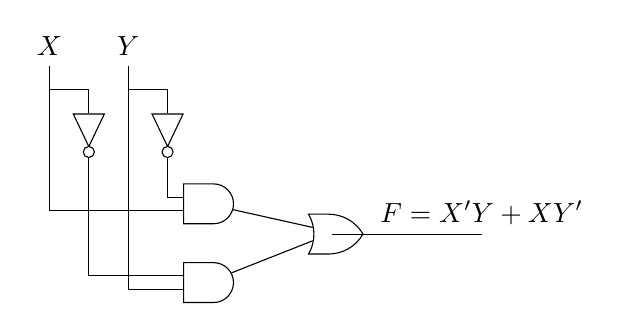
\begin{tikzpicture}[label distance=2mm]

    \node (X) at (0,0) {$X$};
    \node (Y) at (1,0) {$Y$};
     \node[not gate US, draw, rotate=-90] at ($(X)+(0.5,-1)$) (not1) {};
    \node[not gate US, draw, rotate=-90] at ($(Y)+(0.5,-1)$) (not2) {};
    \node[and gate US, draw, logic gate inputs=nn] at ($(X)+(2,-2)$) (and1) {};
    \node[and gate US, draw, logic gate inputs=nn] at ($(and1)+(0,-1)$) (and2) {};
    \node[or gate US, draw, logic gate inputs=nn, anchor=input 1] at ($(and1.output)+(1,-0.3)$) (or1) {};
    \draw (X) |- (and1.input 2);
    \draw (Y) |- (and2.input 2);
    \draw (and1) -- (or1.input 1);
    \draw (and2) -- (or1.input 2);
    \draw (not1) |- (and2.input 1);
    \draw (not2) |- (and1.input 1);
    \draw (or1) |- (or1.output);
    \path (X) -- coordinate (punt)(X |- not1.input);
    \draw (punt)-| (not1.input);
    \path (Y) -- coordinate (punt)(Y |- not2.input);
    \draw (punt) -| (not2.input);
    \draw (or1.output) -- ([xshift=1.5cm]or1.output) node[above] {$F=X'Y +XY'$};
    \end{tikzpicture} 
\begin{center}
    Figure 1
\end{center}
\end{document}